\chapter{Architektura Ansible}\label{sec:ansible}
V~Ansible jsou pro definici konfigurace a~automatizačních úloh nejčastěji používány strukturované formáty YAML, INI a~šablonovací jazyk Jinja2.
\begin{itemize}
    \item \textbf{YAML} \\
    YAML (YAML Ain't Markup Language) je formát pro serializaci dat, který je navržen tak, aby byl snadno čitelný pro lidi a~zároveň snadno zpracovatelný počítači.
    \cite{yamldocs}
    \begin{lstlisting}[language=YAML, caption={Ukázka YAML}, label={lst:yamlshowcase}, captionpos=b]
    general:
        name: TestApp
        version: 1.0

    settings:
        theme: dark
        lang: cs
    \end{lstlisting}
    \item \textbf{INI} \\
    INI je jednoduchý formát pro konfigurační soubory, který používá strukturu klíč-hodnota a~sekce pro organizaci nastavení.
        
    \begin{lstlisting}[caption={Ukázka INI}, label={lst:inishowcase}, captionpos=b]
    [General]
    name=TestApp
    version=1.0

    [Settings]
    theme=dark
    lang=cs
    \end{lstlisting}

    \item \textbf{Jinja2} \\
    Jinja2 je šablonovací jazyk pro Python, který umožňuje generovat textové soubory na základě šablon a~proměnných.
    \cite{jinja2docs}
    \clearpage
    \begin{lstlisting}[language={}, caption={Ukázka Jinja2}, label={lst:jinjashowcase}, captionpos=b]
    Application: {{ name }}
    Version: {{ version }}

    Language: {{ lang }}
    Theme: {{ theme }}
    \end{lstlisting}
   
\end{itemize}
Tyto formáty tvoří základ pro hlavní části konfigurace, jako jsou playbooky, inventáře a~šablony. 
Kromě nich však mohou být v~rámci Ansible projektů využívány také další typy souborů, například skripty v~jazycích Bash nebo Python, či~statické datové soubory (např. JSON nebo CSV), které slouží jako doplňkové zdroje dat.
\cite{ansibledocs}

Samotná struktura Ansible projektu je následně rozdělena do několika klíčových komponent:
\begin{itemize}
    \item \textbf{Řídicí uzel} \\
    Řídící uzel je stroj, na kterém je nainstalován Ansible a~odkud jsou spouštěny všechny automatizační úlohy.
    Obsahuje veškeré konfigurační soubory, playbooky a~inventáře cílových uzlů. \cite{ansibledocs}

    \item \textbf{Řízené uzly} \\
    Řízené uzly jsou servery nebo zařízení, která Ansible spravuje. Mohou to být například fyzické servery, virtuální stroje, kontejnery nebo síťová zařízení.
    
    Ansible komunikuje s~těmito uzly hlavně pomocí protokolu SSH a~provádí na nich definované úlohy.
    Existují ale i~jiné způsoby komunikace, například \texttt{local} pro lokální operace nebo \texttt{docker} pro správu Docker kontejnerů. \cite{ansibledocs}
    
    V~Ansible se dá připojit ať už k~jednomu nebo více řízeným uzlům najednou. Pokud není specifikováno jinak, tak paralelně. 
    Tyto skupiny jsou definovány v~inventáři.
    \item \textbf{Task} \\
    Task, neboli úloha, je základní jednotka práce v~Ansible, která definuje konkrétní akci, kterou má Ansible provést na řízeném uzlu.
    Úlohy jsou definovány v~playboocích a~mohou zahrnovat různé operace, jako je instalace softwaru, kopírování souborů, 
    spouštění příkazů nebo konfigurace služeb. \cite{ansibledocs}
    \begin{lstlisting}[language=YAML, caption={Ansible - ukázka úlohy (Task)}, label={lst:ansibletask}, captionpos=b]
    - name: Ensure postgresql is at the latest version
      ansible.builtin.yum:
        name: postgresql
        state: latest
    \end{lstlisting}

    \item \textbf{Playbook} \\
    Playbooky jsou soubory ve formátu YAML, které obsahují sadu úloh pro Ansible.
    Definují, jaké úlohy mají být provedeny na kterých řízených uzlech a~v~jakém pořadí.
    Playbooky umožňují automatatizovat složité procesy a~zajišťují opakovatelnost a~konzistenci konfigurací. \cite{ansibledocs}
    \begin{lstlisting}[language=YAML, caption={Ansible - ukázka playbooku}, label={lst:ansibleplaybook}, captionpos=b]
    ---
    - name: Update db servers
      hosts: dbservers
      remote_user: root

      tasks:
        - name: Ensure postgresql is at the latest version
          ansible.builtin.yum:
            name: postgresql
            state: latest

        - name: Ensure that postgresql is started
          ansible.builtin.service:
            name: postgresql
            state: started
    \end{lstlisting}


    \item \textbf{Modul} \\
    Moduly představují základní vykonávací jednotky v~Ansible. Každá úloha (\textit{task}) v~playbooku využívá některý 
    modul k~provedení konkrétní operace na řízeném uzlu. Modul tedy definuje, jaký typ akce má být vykonán.
    
    Ansible obsahuje velké množství vestavěných modulů, které jsou dostupné v~tzv. \textit{kolekcích}. 
    Nejčastěji používané vestavěné moduly se nacházejí v~kolekci \texttt{ansible.builtin}, například:

    \begin{itemize}
        \item \texttt{ansible.builtin.copy} – kopírování souborů mezi řídicím a~řízeným uzlem,
        \item \texttt{ansible.builtin.user} – správa uživatelských účtů na řízeném uzlu,
        \item \texttt{ansible.builtin.service} – správa systémových služeb (start, stop, restart),
    \end{itemize}

    Lze najít a~stáhnout i~moduly z~externích modulovacích kolekcí. \cite{ansibledocs}
    \item \textbf{Inventář} \\
    Inventář je soubor, který obsahuje seznam řízených uzlů, které Ansible spravuje.
    Může být ve formátu INI, nebo YAML a~buď statický, předem sestavený, nebo dynamický, vygenerovaný skriptem.
    Inventář umožňuje organizovat uzly do skupin, což usnadňuje cílení úloh na specifické sady zařízení. \cite{ansibledocs}
    \clearpage
    \begin{lstlisting}[caption={Ansible - ukázka INI inventáře}, label={lst:ansibleiniinventory}, captionpos=b]
    mail.example.com

    [webservers]
    foo.example.com
    bar.example.com

    [dbservers]
    one.example.com
    two.example.com
    192.168.1.200
    \end{lstlisting}

    \begin{lstlisting}[language=YAML, caption={Ansible - ukázka YAML inventáře}, label={lst:ansibleyamlinventory}, captionpos=b]
    ungrouped:
        hosts:
            mail.example.com:
    webservers:
        hosts:
            foo.example.com:
            bar.example.com:
    dbservers:
        hosts:
            one.example.com:
            two.example.com:
            192.168.1.200:
    \end{lstlisting}

    Ansible definuje vždy 2 hlavní seskupení v~inventáři: 
    \begin{itemize}
        \item \texttt{all} - obsahuje všechny zařízení v~inventáři
        \item \texttt{ungrouped} - obsahuje zařízení, které nejsou přiřazeny do žádné skupiny
    \end{itemize}
    Všechny ostatní skupiny jsou definovány uživatelem a~mohou být hierarchicky organizovány, což umožňuje vytvářet podskupiny a~dědit vlastnosti mezi skupinami. \cite{ansibledocs}


    \item \textbf{Role} \\
    Role jsou způsob, jak organizovat playbooky a~úlohy do znovupoužitelných komponent.
    Takto vytvořené role mohou být dále znovu použity a~také sdíleny přes Ansible Galaxy.
    Role umožňují strukturovat kód do předem definovaných adresářů, které vypadají následovně:
    \clearpage
    \begin{lstlisting}[language=YAML, caption={Struktura adresářů pro Ansible role}, label={lst:ansiblerole}, captionpos=b]
        roles/
            common/
                tasks/
                    main.yml
                handlers/
                    main.yml 
                templates/
                    ntp.conf.j2
                files/
                    bar.txt
                    foo.sh
                vars/
                    main.yml
                defaults/
                    main.yml
                meta/
                    main.yml
                library/
                module_utils/
                lookup_plugins/

            webtier/
            monitoring/
            fooapp/
    \end{lstlisting} 

    Jednotlivé adresáře v~roli mají specifický účel:
    \begin{itemize}
        \item \textbf{tasks} - obsahuje hlavní úlohy, které se mají provést, obvykle v~souboru \texttt{main.yml}
        \item \textbf{handlers} - obsahuje úlohy, které se spustí pouze v~případě, že jsou "vyvolány" z~jiných úloh, například pro restart služby po změně konfigurace
        \item \textbf{templates} - obsahuje šablony, které se používají pro generování konfiguračních souborů na základě proměnných
        \item \textbf{files} - obsahuje statické soubory, které se mají zkopírovat na řízené uzly
        \item \textbf{vars} - obsahuje proměnné, které se mají použít v~souboru \texttt{main.yml}
        \item \textbf{defaults} - obsahuje proměnné, které se mají použít v~souboru \texttt{main.yml}, ale s~nižší prioritou než proměnné v~adresáři~\texttt{vars}
        \item \textbf{meta} - obsahuje metadata o~roli, jako jsou závislosti na jiných rolích
        \item \textbf{library} - obsahuje vlastní moduly, které mohou být použity v~úlohách
        \item \textbf{module\_utils} - obsahuje pomocné funkce pro vlastní moduly
        \item \textbf{lookup\_plugins} - obsahuje vlastní lookup pluginy, které umožňují získávat data z~různých zdrojů
    \end{itemize}

    \item \textbf{Proměnná} \\
    Proměnné v~Ansible umožňují ukládat hodnoty, které lze použít v~různých částech playbooku. 
    Tyto proměnné mohou být definovány na různých místech v~projektu, a~podle toho mají i~přiřazené priority, pro případ kdyby se proměnné jmenovaly stejně (např. při~definování výchozí cesty k~souboru s~konfigurací).  \cite{ansibledocs}

    Název proměnných je pouze omezen tím, že musí začínat písmenem nebo podtržítkem a~může obsahovat pouze alfanumerické znaky a~podtržítka.
    Dále jsou některé názvy proměnných rezervované, například \texttt{ansible\_facts} nebo \texttt{inventory\_hostname}. \cite{ansibledocs}
    
    Proměnné se používají pomocí šablonovacího systému Jinja2, který umožňuje vkládat proměnné do textu a~také provádět různé operace s~nimi, jako jsou podmínky, smyčky nebo filtry.
    Aby Ansible věděl, že se jedná o~proměnnou, musí být její název obklopen dvojitými složenými závorkami a~uzavřen v~uvozovkách, například \texttt{"\{\{ promenna \}\}"}. \cite{ansibledocs}

    \begin{lstlisting}[language=YAML, caption={Použití proměnné}, label={lst:ansiblepromennapouziti}, captionpos=b]
    - debug:
        msg: "Hodnota je {{ promenna }}"
    \end{lstlisting}

    \begin{itemize}
        \item \textbf{Fakta} \\
        Specifickým typem proměnných jsou tzv. "fakta", které Ansible automaticky shromažďuje o~cílových uzlech během běhu playbooku.
        
        Přistupuje se k~nim přes proměnnou \texttt{ansible\_facts} a~obsahují informace o~hardwaru, operačním systému, síťových rozhraních a~dalších charakteristikách uzlu.
        K~některým faktům lze přistupovat i~zkráceně, například \texttt{ansible\_facts['os\_family']} lze zapsat jako \texttt{ansible\_os\_family}. \cite{ansibledocs}
         
        \begin{lstlisting}[language=YAML, caption={Shromážděná fakta}, label={lst:ansiblefacts}, captionpos=b]
        {
        "ansible_all_ipv4_addresses": [
            "192.168.1.2"
        ],
        "ansible_all_ipv6_addresses": [
            "2345:0425:2CA1:0000:0000:0567:5673:23b5"
        ],
        "ansible_apparmor": {
            "status": "disabled"
        },
        "ansible_architecture": "x86_64",
        ...
        }
        \end{lstlisting}

        Shromažďování faktů lze ovlivnit pomocí proměnné \texttt{gather\_facts}, která se nastavuje na úrovni playbooku.
        Jejich kolekce může pro některé případy být zbytečná a~velmi zpomalovat průběh playbooku. \cite{ansibledocs}
    \end{itemize}

    Při~kolizi názvů proměnných se použije následující neuplný výčet priority (vyšší číslo znamená vyšší prioritu):
    \begin{enumerate}
        \item \textbf{Proměnné přidané argumentem}
        \begin{lstlisting}[language=YAML, caption={Proměnné přidané argumentem}, label={lst:ansibleargumentvar}, captionpos=b]
        ansible-playbook playbook.yml -e "promenna=foo"
        \end{lstlisting}

        \item \textbf{Proměnné role} \\
            Proměnné definované ve \texttt{roles/myrole/vars/main.yml}.
            Na stejné úrovni jsou i~proměnné definované při~zahrnutí role v~playbooku.
            \begin{lstlisting}[language=YAML, caption={Proměnné při~zahrnutí role}, label={lst:ansiblerolevar}, captionpos=b]
            - roles:
                - role: myrole
                  vars: 
                      promenna: foo
            \end{lstlisting}

        \item \textbf{Registrované proměnné}
        \begin{lstlisting}[language=YAML, caption={Registrované proměnné}, label={lst:ansibleregisteredvar}, captionpos=b]
        - command: echo hello
        register: promenna
        \end{lstlisting}
        Tyto proměnné jsou vytvořeny během běhu playbooku a~obsahují výsledky z~úloh, které je vytvořily. 
        Využívají se například pro kontrolu úspěšného provedení úlohy nebo pro získání výstupu z~příkazu.

        \item \textbf{Playbook proměnné} \\
        Proměnné definované přímo v~souboru \texttt{playbook.yml}.
        \begin{lstlisting}[language=YAML, caption={Playbook proměnné}, label={lst:ansibleplaybookvar}, captionpos=b]
        - hosts: all
          vars:
              promenna: foo
          tasks:
              ...
        \end{lstlisting}

        \item \textbf{Host\_vars proměnné} \\
        Proměnné definované pro konkrétní hosty v~adresáři~\texttt{host\_vars/}. 
        Každý soubor v~tomto adresáři~je pojmenován podle názvu hosta, pro který jsou proměnné určeny.
        \begin{lstlisting}[language=YAML, caption={Proměnné hostů}, label={lst:ansiblehostvars}, captionpos=b]
        # host_vars/server1.yml
        promenna: foo
        \end{lstlisting}

        \item \textbf{Group\_vars proměnné} \\
        Proměnné definované pro skupiny hostů v~adresáři~\texttt{group\_vars/}. 
        Každý soubor v~tomto adresáři~je pojmenován podle názvu skupiny, pro kterou jsou proměnné určeny.
        \begin{lstlisting}[language=YAML, caption={Proměnné skupin}, label={lst:ansiblegroupvars}, captionpos=b]
        # group_vars/web.yml
        promenna: foo
        \end{lstlisting}

        \item \textbf{Proměnné v~inventáři} \\
        Proměnné definované přímo v~inventářním souboru. 
        Může se jednat o~proměnné pro konkrétní hosty nebo pro celé skupiny podle umístění. 
        Využívají se například pro definování specifických nastavení pro jednotlivé skupiny, jako je např. styl připojení.
        \begin{lstlisting}[language=YAML, caption={Proměnné v~inventáři}, label={lst:ansibleinventoryvar}, captionpos=b]
        [web]
        server1 promenna=foo
        \end{lstlisting}

        \item \textbf{Fakta}\\
        Automaticky shromážděné informace o~cílových uzlech, přístupné přes proměnnou \texttt{ansible\_facts}.
        
        \item \textbf{Výchozí proměnné role} \\
        Definované v~\texttt{roles/myrole/defaults/main.yml}. Absolutně nejnižší priorita.
    \end{enumerate}
    
    Citlivé proměnné, jako jsou hesla nebo klíče, by měly být šifrovány pomocí Ansible Vault, což je nástroj pro zabezpečení dat v~Ansible. 
    
    Ten ale zabezpečuje data jen v~případě "data at rest", to znamená uložená data v~souborech. 
    Jakmile jsou data během běhu playbooku dešifrována, nacházejí se v~paměti a~mohou být zobrazeny ve výstupu. 
    Proto je vhodné citlivé informace skrýt pomocí parametru \texttt{no\_log}, který zabrání jejich zobrazení ve výstupu playbooku.  \cite{ansibledocs}
\end{itemize}

\chapter{Architektura Prometheus}\label{sec:prometheus}
Prometheus se konfiguruje pomocí YAML souboru, kde se definují zdroje dat, pravidla pro shromažďování metrik a~nastavení upozornění.
\begin{lstlisting}[language=YAML, caption={Prometheus - ukázka konfigurace}, label={lst:prometheusconfig}, captionpos=b]
global:
    scrape_interval: 15s
    evaluation_interval: 15s

rule_files:
    - "alert.rules"

scrape_configs:
- job_name: prometheus
    static_configs:
    - targets: ['localhost:9090']
\end{lstlisting}

Existují zde 3 hlavní bloky:
\begin{itemize}
    \item \textbf{global} - obsahuje globální nastavení pro Prometheus, jako je interval shromažďování dat a~interval vyhodnocování pravidel pro upozornění.
    \item \textbf{rule\_files} - obsahuje seznam souborů s~pravidly pro upozornění, které definují podmínky, za kterých má být odesláno upozornění.
    \item \textbf{scrape\_configs} - obsahuje konfigurace pro shromažďování dat z~různých zdrojů, včetně názvu úlohy a~seznamu cílů, ze kterých se mají data shromažďovat.
\end{itemize}

\subsubsection{Datový Model}
Prometheus ukládá data ve formě časových řad.

\begin{itemize}
    \item \textbf{Metrika} - základní jednotka dat, která představuje konkrétní sadu měření, například \texttt{http\_requests\_total} pro počet HTTP požadavků.
    \item \textbf{Štítek} - klíč-hodnota pár, který poskytují další kontextové informace o~metrice.
    \item \textbf{Hodnota} - konkrétní měření pro danou metriku a~sadu štítků, například počet požadavků v~určitém časovém okamžiku.
\end{itemize}

Dále se jednotlivé metriky dělí do 4 typů:
\begin{itemize}
    \item \textbf{Counter} \\
    Monotonicky rostoucí hodnota, která se zvyšuje pouze při~události, například počet požadavků.
    \begin{figure}[H]
        \centering
        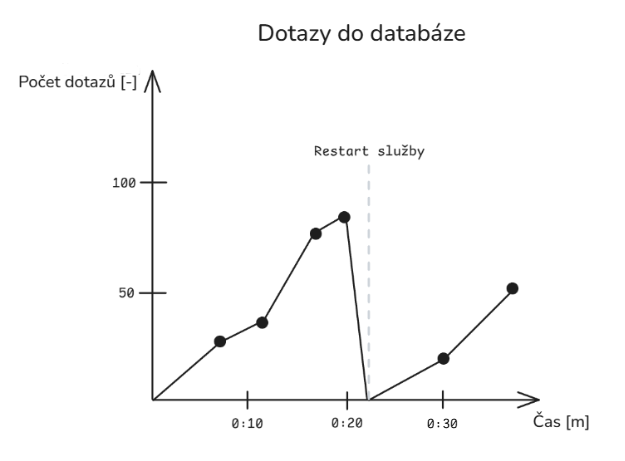
\includegraphics[width=0.7\textwidth]{images/counter.png}
        \caption{Ukázka metriky typu Counter (zdroj: vlastní zpracování)}
        \label{fig:counter}
    \end{figure}
    \item \textbf{Gauge} \\ 
    Hodnota, která může růst i~klesat, například aktuální využití CPU.
    \begin{figure}[H]
        \centering
        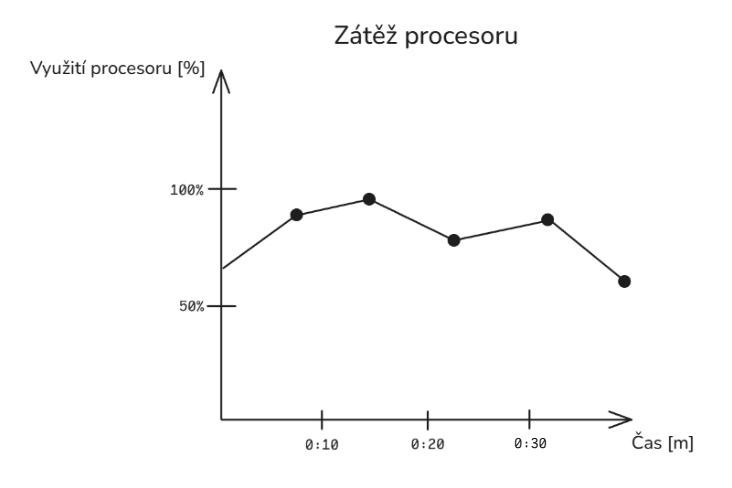
\includegraphics[width=0.8\textwidth]{images/gauge.png}
        \caption{Ukázka metriky typu Gauge (zdroj: vlastní zpracování)}
        \label{fig:gauge}
    \end{figure}    
    \item \textbf{Histogram} \\
    Měří distribuci hodnot, například doby odezvy, a~poskytuje informace o~počtu vzorků a~součtech pro různé intervaly.
    \begin{figure}[H]
        \centering
        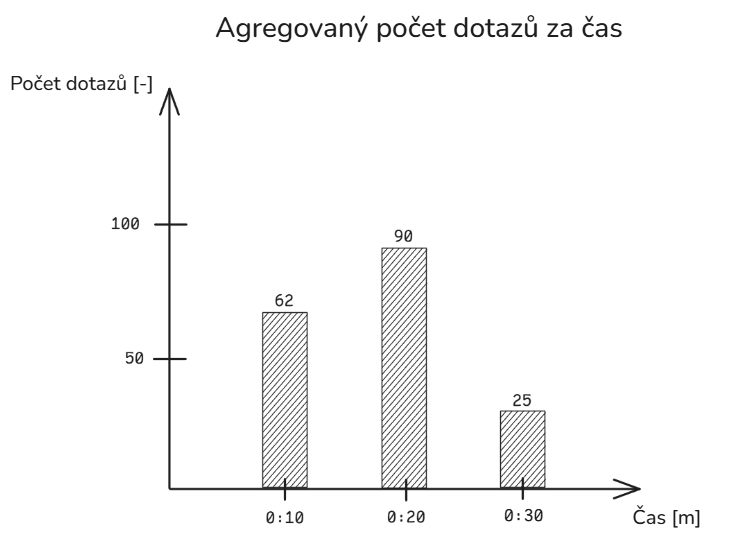
\includegraphics[width=0.8\textwidth]{images/histogram.png}
        \caption{Ukázka metriky typu Histogram (zdroj: vlastní zpracování)}
        \label{fig:histogram}
    \end{figure}
    \item \textbf{Summary} \\ 
    Podobný histogramu, ale poskytuje kvantily pro měření distribuce, například 95. percentil doby odezvy.
\end{itemize}   

\subsubsection{PromQL}
PromQL, celým názvem Prometheus Query Language, je dotazovací jazyk pro Prometheus.
Dotazy mohou být buď "instantní", které vracejí aktuální hodnoty metrik, nebo "časový rozsah", které vracejí historické hodnoty pro zadané časové období. \cite{prometheusdocs}
\begin{lstlisting}[language=promql, caption={PromQL - ukázka dotazů}, label={lst:promql}, captionpos=b]
    rate(http_requests_total[5m])[30m:1m]
\end{lstlisting}
Tento dotaz vrací rychlost změny metriky \texttt{http\_requests\_total} za posledních 5 minut, přičemž se tato rychlost počítá pro každou minutu v~posledních 30 minutách.
\clearpage
\subsubsection{Node Exporter}
Node Exporter je nástroj pro sběr systémových metrik z~hostitelského systému, který je monitorován pomocí Prometheus.
Node Exporter shromažďuje informace o~specifickém systému pro který je konfigurován, například o~CPU, paměti, disku, síti a~dalších hardwarových a~systémových parametrech. \cite{prometheusdocs}

Je třeba ho distribuovat a~spustit na každém hostitelském systému, který chceme monitorovat, a~poté nakonfigurovat Prometheus, aby shromažďoval data z~těchto Node Exporterů. \cite{prometheusdocs}
\subsubsection{Alertmanager}
Alertmanager je komponenta Prometheus, která se stará o~správu a~odesílání upozornění.
Umožňuje definovat pravidla pro upozornění, která se spouštějí na základě dotazů PromQL, a~poté odesílat upozornění prostřednictvím různých kanálů, jako jsou e-mail, Slack a~další. \cite{prometheusdocs}

\chapter{Externí přílohy\label{sec:ep}}

Externí přílohy této bakalářské práce jsou umístěny na adrese:\\ \url{https://github.com/Jiri-Fiser/thesis_ki_ujep}.

Na úložiští GitHub mohou byt uloženy tyto externí přílohy:

\begin{itemize}
\item \textbf{zdrojové kódy}
\item \textbf{doplňkové texty} (například jak instalovat aplikaci, manuály aplikace)
\item \textbf{schémata} (především, pokud se nevejdou na stranu A4 a~jejich vytištění je tak problematické)
\item \textbf{screenshoty} (v~textu práce lze použít jen omezený počet snímků obrazovky, které navíc nemusí být při~černobílém tisku příliš přehledné)
\item \textbf{videa} (například ovládání aplikace)
\end{itemize}

V~každém případě by to však měli být pouze materiály, které jste vytvořili sami. Materiály jiných autorů uvádějte v~seznamu použité literatury (včetně případných odkazů na jejich originální umístění).

V~této kapitole stačí uvést pouze základní strukturu úložiště (co se kde nalézá a~jakou má funkci) například v~podobě tabulky. 

\begin{longtable}{ll}
\hline
ki-thesis.pdf & text práce v~PDF \\
ki-thesis.tex & zdrojový kód práce v~\LaTeX{}u~\\
kitheses.cls & definice třídy dokumentů (rozšířená třída \texttt{scrbook} \\
thesis.bib & bibliografická databáze (exportována z~citace.com) \\
LOGO\_PRF\_CZ\_RGB\_standard.jpg  & logo fakulty s~českým textem \\
LOGO\_PRF\_EM\_RGB\_standard.jpg  & logo fakulty s~anglickým textem  \\
\hline
\end{longtable}

Všechny tyto soubory jsou potřeba pro překlad dokumentu (logo stačí jedno v~příslušné jazykové verzi).